%% Based on a TeXnicCenter-Template by Gyorgy SZEIDL.
%%%%%%%%%%%%%%%%%%%%%%%%%%%%%%%%%%%%%%%%%%%%%%%%%%%%%%%%%%%%%

%----------------------------------------------------------
%
\documentclass[a4paper,11pt,twoside]{report}
%
%----------------------------------------------------------
% This is a sample document for the standard LaTeX Report Class
% Class options
%       --  Body text point size:
%                        10pt (default), 11pt, 12pt
%       --  Paper size:  letterpaper (8.5x11 inch, default)
%                        a4paper, a5paper, b5paper,
%                       legalpaper, executivepaper
%       --  Orientation (portrait is the default):
%                       landscape
%       --  Printside:  oneside (default), twoside
%       --  Quality:    final (default), draft
%       --  Title page: titlepage, notitlepage
%       --  Columns:    onecolumn (default), twocolumn
%       --  Start chapter on left:
%                       openright(no), openany (default)
%       --  Equation numbering (equation numbers on right is the default)
%                       leqno
%       --  Displayed equations (centered is the default)
%                       fleqn (flush left)
%       --  Open bibliography style (closed bibliography is the default)
%                       openbib
% For instance the command
%          \documentclass[a4paper,12p,leqno]{report}
% ensures that the paper size is a4, fonts are typeset at the size 12p
% and the equation numbers are on the left side.
%
\usepackage{amsmath}
\usepackage{amsfonts}
\usepackage{amssymb}
\usepackage{graphicx}
\usepackage{url}
\usepackage{listings} %Per inserire codice
\usepackage[usenames]{color}
%----------------------------------------------------------

%----------------------------------------------------------
\begin{document}

\begin{titlepage}
	\centering
	
\includegraphics[scale = 0.4]{logo.jpeg}\\[1.0 cm]
	\textsc{\LARGE University of Pavia}\\[1.0 cm]
	\textsc{\Large Advanced Computer Architecture}\\[0.5 cm]
	\rule{\linewidth}{0.2 mm} \\[0.4 cm]
	{\huge{\textbf{Game of Life 2D}}}\\
	\rule{\linewidth}{0.2 mm} \\[1 cm]

	{\large Federica Amato, Andrea Bonandin} \\[0.2 cm]
	\url{federica.amato02@universitadipavia.it}
	\url{andrea.bonandin01@universitadipavia.it} \\[0.2 cm]
	{February 2017}
\end{titlepage}

\tableofcontents

\chapter{Introduction}
In the 1940s, the physicist and mathematician John Von Neumann began working
on the solution of the mystery of self-reproduction as employed in biological systems. He was
interested in the use of computing devices to model the complex behavior of organisms.
Von Neumann was determined to answer the question, "What kind of logical organization is sufficient for an automaton to be able to reproduce itself?" He proposed a solution to this question in
his book Theory of Self-Reproducing Automata (completed and published in 1966).

\noindent Since then, cellular automata have been used in a variety of ways and have taken on multiple definitions, but it is generally agreed upon that all cellular automata consist of a collection of 'colored' cells on a grid of specified shape, that evolves through a number of discrete time steps according to a set of rules based on the states of neighboring cells. As such, every cellular automata consists of a certain type of cellular space and a transition rule. The cellular space can
be described in terms of any d-dimensional regular lattice of cells with finite boundary conditions.
Each cell has $k $number of states where $k$ is most commonly used as a positive integer ($k : k \in Z+$). The set of states is denoted $\sum$ , making $k = |\sum|$. 

\chapter{Conway's Game of Life}\label{Conway}

In the 1970s, Cambridge Professor John Conway invented a 2-dimensional cellular automaton consisting of a Moore neighborhood that he called "life". In doing so, he was hoping to be able to study the macroscopic behaviors of a population.

\noindent The "game" is a zero-player game, meaning that its evolution is determined by its initial state, requiring no further input. One interacts with the Game of Life by creating an initial configuration and observing how it evolves, or, for advanced "players", by creating patterns with particular properties.

\section{Basic Rules}
Conway experimented with various transition rules and eventually decided on this setup:
\begin{itemize}

	\item $\sum = \{0, 1\}$ where a state of 0 represents a dead member of the population    and 1 represents an alive member of the population;
	\item The transition rule consists of either the death of a member (going from $1 \rightarrow 0$), birth of a member ($0 \rightarrow 1$), or no change ($0 \rightarrow 0$ or $1 \rightarrow 1$);
	\item With zero or one bordering member alive in a cells neighborhood, death occurs due to loneliness;
	\item With two or three members alive in the neighborhood, there is no change to an alive member;
	\item If a dead member's neighborhood consists of three live members, a new member is born ($0 \rightarrow 1$);
	\item If a live member's neighborhood consists of more than three live members, it will die due to overpopulation.
\end{itemize}


\chapter {Serial Code Analysis}

In our code, the world of Game of Life is represented by a rectangular grid where there are ones and zeroes. Zeroes represent dead cells instead ones represent cells which are alive. We decided to use toroidal boundary conditions such that no cell could vanish going out from the grid.

\noindent To realize the Conway's Game of Life, we are inspired by the Serial code found in \cite{code}.

\noindent We decided to change the code found to improve performance and modularity. 
So we managed matrices using a single array to take advantage of the principle of locality of access and we divided the code into three principle functions:  
\begin{itemize}

	\item \emph{init}: it initializes the matrix with two additional rows and columns set to zero to represent boundaries and sets with zero or one random values the internal grid.
	\item \emph{evolve}: after setting boundary conditions, it checks the numbers of neighbors and   
	sets the new cell's state in a second array according with the rules explained in chapter \ref{Conway}.
	\item \emph{update}: it changes the original array with the new calculated in evolve.

\end{itemize}

\noindent After the allocation of two empty array (one for the actual state and one for the successive), the init function is called, then we enter in a cycle which continues evolving and updating the grid, starting from the initialized array until the set number of generations (see Figure \ref{fig:1} .
To debug the program we used also a show function which prints the array. 

\noindent However this approach is possible only for small grids and it is not useful for performance measurements. So in the final code is not present.

\begin{figure}
	\centering
	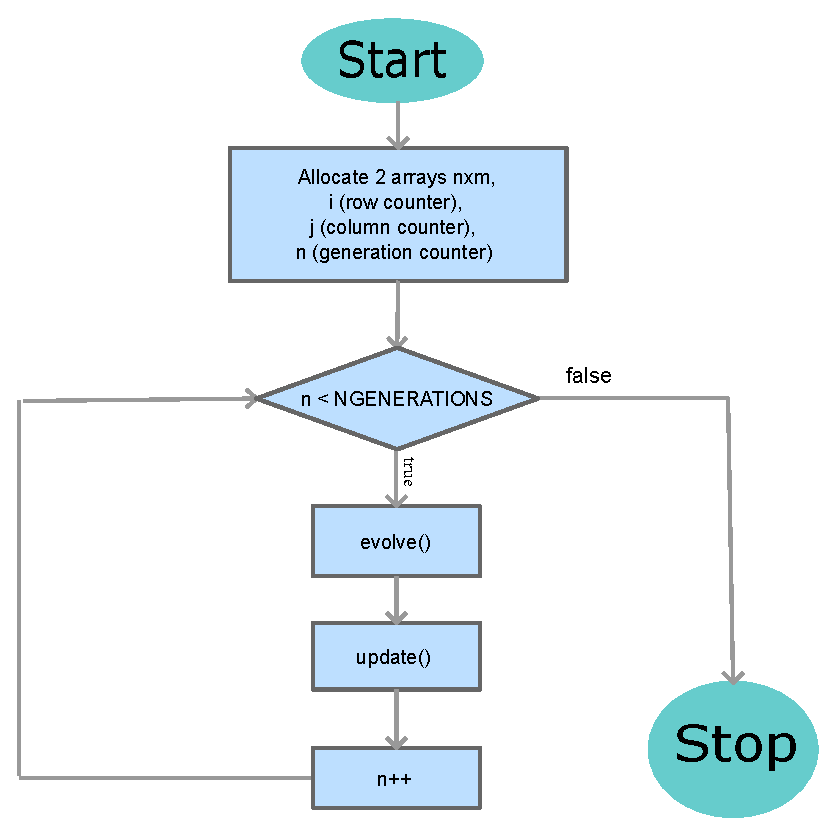
\includegraphics[scale = 0.8]{chart.eps}
	\caption{\emph{Game of Life's flowchart}}\label{fig:1}
\end{figure}	


\appendix



\chapter{Serial Code}





\chapter{Parallel Code}



\begin{thebibliography}{9}
\bibitem {Life} Caleb Koch, "Regularity in Conway's Game of Life", 2015
\bibitem {wiki} Web, \url{https://en.wikipedia.org/wiki/Conway's_Game_of_Life}
\bibitem {stan} Web, \url{http://web.stanford.edu/~cdebs/GameOfLife}
\bibitem {code} Web, \url{https://www.pdc.kth.se/education/tutorials/summer-school/mpi-exercises/mpi-lab-codes/game_of_life-serial.c/view}
\end{thebibliography}
\end{document}

\end{document}
